%  LaTeX support: latex@mdpi.com
%  In case you need support, please attach all files that are necessary for compiling as well as the log file, and specify the details of your LaTeX setup (which operating system and LaTeX version / tools you are using).

%=================================================================
\RequirePackage{fix-cm}
\RequirePackage{amsmath}
% \documentclass[journal,article,accept,moreauthors,pdftex]{Definitions/mdpi}
\documentclass[preprints,article,accept,moreauthors,pdftex]{Definitions/mdpi}

\newcommand\notsotiny{\@setfontsize\notsotiny{6}{7}}
\usepackage[T1]{fontenc}% optional T1 font encoding
\usepackage{datetime,xcolor,etoolbox}
\usepackage{etoolbox}
%\usepackage{xcolor}
\usepackage{soul}
\soulregister\cite7

% Some very useful LaTeX packages include:
% (uncomment the ones you want to load)
\usepackage[font=scriptsize,labelfont=bf]{caption}
\usepackage{amsmath,amssymb,amsfonts}
% \usepackage{amsfonts} % to load math symbols
\usepackage{commath} % For defining functions
%\usepackage{mdwmath}
\usepackage[nolist]{acronym}
% \usepackage{showframe}\\

\usepackage{graphicx}
\usepackage{color}
\usepackage{subfig}
\usepackage{caption}
% % The following is done to hide ugly color boxes around the links
\usepackage[table]{xcolor}
\usepackage{times}
\usepackage{booktabs}
\usepackage{float}
\usepackage{newtxtext,newtxmath}
\usepackage{tabularx,colortbl}
\usepackage{pgfplots}
\usepackage{standalone}
\usepackage{tikz}
\tikzset{
	font={\fontsize{8pt}{8}\selectfont}}
\usepackage{tikzscale} % Scale the figure not the font
\pgfplotsset{compat=newest}
%% the following commands are sometimes needed
\usepackage{grffile}
\usepackage{mathtools}
\usepackage[separate-uncertainty = true,
	multi-part-units = repeat]{siunitx}
\sisetup{per=slash, load=abbr, output-complex-root = j, complex-root-position = before-number}

% declare the path(s) where your graphic files are
\graphicspath{{Figures/}}
%
% Personal definitions
\renewcommand{\v}[1]{\mathbf{#1}} % vectors
\newcommand{\ti}[1]{\tilde{#1}} % spectral representation
\newcommand{\tnsr}[1]{\underline{\underline{#1}}}
% Operators
\renewcommand{\O}{\omega}  % omega
\newcommand{\E}{\varepsilon}  % epsilon
\renewcommand{\u}{\mu}  % mu
\newcommand{\p}{\rho}  % rho
\newcommand{\vp}{\boldsymbol \p}  % rho
\newcommand{\x}{\times}  % times
\renewcommand{\inf}{\infty}  % infinity
\newcommand{\infint}{\int\limits_{-\inf}^\inf} % integral by R
\renewcommand{\del}{\nabla}  % nabla operator
\renewcommand{\^}{\hat}  % unit vector
\newcommand*\diff{\mathop{}\!\mathrm{d}} % Define differential operator
\newcommand{\e}{\mathrm{e}} % Straight-up exponential
\renewcommand{\j}{{j}\mkern1mu} % Straight-up exponential
\newcommand{\iu}{\mathrm{i}\mkern1mu}
% *** Do not adjust lengths that control margins, column widths, etc. ***
% *** Do not use packages that alter fonts (such as pslatex).         ***
% correct bad hyphenation here
\hyphenation{op-tical net-works semi-conduc-tor}
%

% If you would like to post an early version of this manuscript as a preprint, you may use preprint as the journal and change 'submit' to 'accept'. The document class line would be, e.g., \documentclass[preprints,article,accept,moreauthors,pdftex]{mdpi}. This is especially recommended for submission to arXiv, where line numbers should be removed before posting. For preprints.org, the editorial staff will make this change immediately prior to posting.

%--------------------
% Class Options:
%--------------------
%----------
% journal
%----------
% Choose between the following MDPI journals:
% acoustics, actuators, addictions, admsci, aerospace, agriculture, agriengineering, agronomy, algorithms, animals, antibiotics, antibodies, antioxidants, applsci, arts, asc, asi, atmosphere, atoms, axioms, batteries, bdcc, behavsci , beverages, bioengineering, biology, biomedicines, biomimetics, biomolecules, biosensors, brainsci , buildings, cancers, carbon , catalysts, cells, ceramics, challenges, chemengineering, chemistry, chemosensors, children, cleantechnol, climate, clockssleep, cmd, coatings, colloids, computation, computers, condensedmatter, cosmetics, cryptography, crystals, dairy, data, dentistry, designs , diagnostics, diseases, diversity, drones, econometrics, economies, education, ejihpe, electrochem, electronics, energies, entropy, environments, epigenomes, est, fermentation, fibers, fire, fishes, fluids, foods, forecasting, forests, fractalfract, futureinternet, futurephys, galaxies, games, gastrointestdisord, gels, genealogy, genes, geohazards, geosciences, geriatrics, hazardousmatters, healthcare, heritage, highthroughput, horticulturae, humanities, hydrology, ijerph, ijfs, ijgi, ijms, ijns, ijtpp, informatics, information, infrastructures, inorganics, insects, instruments, inventions, iot, j, jcdd, jcm, jcp, jcs, jdb, jfb, jfmk, jimaging, jintelligence, jlpea, jmmp, jmse, jnt, jof, joitmc, jpm, jrfm, jsan, land, languages, laws, life, literature, logistics, lubricants, machines, magnetochemistry, make, marinedrugs, materials, mathematics, mca, medicina, medicines, medsci, membranes, metabolites, metals, microarrays, micromachines, microorganisms, minerals, modelling, molbank, molecules, mps, mti, nanomaterials, ncrna, neuroglia, nitrogen, notspecified, nutrients, ohbm, optics, particles, pathogens, pharmaceuticals, pharmaceutics, pharmacy, philosophies, photonics, physics, plants, plasma, polymers, polysaccharides, preprints , proceedings, processes, proteomes, psych, publications, quantumrep, quaternary, qubs, reactions, recycling, religions, remotesensing, reports, resources, risks, robotics, safety, sci, scipharm, sensors, separations, sexes, signals, sinusitis, smartcities, sna, societies, socsci, soilsystems, sports, standards, stats, surfaces, surgeries, sustainability, symmetry, systems, technologies, test, toxics, toxins, tropicalmed, universe, urbansci, vaccines, vehicles, vetsci, vibration, viruses, vision, water, wem, wevj

%---------
% article
%---------
% The default type of manuscript is "article", but can be replaced by:
% abstract, addendum, article, benchmark, book, bookreview, briefreport, casereport, changes, comment, commentary, communication, conceptpaper, conferenceproceedings, correction, conferencereport, expressionofconcern, extendedabstract, meetingreport, creative, datadescriptor, discussion, editorial, essay, erratum, hypothesis, interestingimages, letter, meetingreport, newbookreceived, obituary, opinion, projectreport, reply, retraction, review, perspective, protocol, shortnote, supfile, technicalnote, viewpoint
% supfile = supplementary materials

%----------
% submit
%----------
% The class option "submit" will be changed to "accept" by the Editorial Office when the paper is accepted. This will only make changes to the frontpage (e.g., the logo of the journal will get visible), the headings, and the copyright information. Also, line numbering will be removed. Journal info and pagination for accepted papers will also be assigned by the Editorial Office.

%------------------
% moreauthors
%------------------
% If there is only one author the class option oneauthor should be used. Otherwise use the class option moreauthors.

%---------
% pdftex
%---------
% The option pdftex is for use with pdfLaTeX. If eps figures are used, remove the option pdftex and use LaTeX and dvi2pdf.

%=================================================================
\firstpage{1}
\makeatletter
\setcounter{page}{\@firstpage}
\makeatother
\pubvolume{xx}
\issuenum{1}
\articlenumber{5}
\pubyear{2019}
\copyrightyear{2019}
%\externaleditor{Academic Editor: name}
\history{Received: date; Accepted: date; Published: date}
%\updates{yes} % If there is an update available, un-comment this line

%% MDPI internal command: uncomment if new journal that already uses continuous page numbers
%\continuouspages{yes}

%------------------------------------------------------------------
% The following line should be uncommented if the LaTeX file is uploaded to arXiv.org
%\pdfoutput=1

%=================================================================
% Add packages and commands here. The following packages are loaded in our class file: fontenc, calc, indentfirst, fancyhdr, graphicx, lastpage, ifthen, lineno, float, amsmath, setspace, enumitem, mathpazo, booktabs, titlesec, etoolbox, amsthm, hyphenat, natbib, hyperref, footmisc, geometry, caption, url, mdframed, tabto, soul, multirow, microtype, tikz

%=================================================================
%% Please use the following mathematics environments: Theorem, Lemma, Corollary, Proposition, Characterization, Property, Problem, Example, ExamplesandDefinitions, Hypothesis, Remark, Definition, Notation, Assumption
%% For proofs, please use the proof environment (the amsthm package is loaded by the MDPI class).

%=================================================================
% Full title of the paper (Capitalized)
\Title{Characterization and Water Content Estimation Method of Living Plant Leaves Using Terahertz Waves}

%% Author Orchid ID: enter ID or remove command
%% Author Orchid ID: enter ID or remove command
\newcommand{\orcidauthorA}{0000-0001-5364-6057}
\newcommand{\orcidauthorB}{0000-0002-5951-9603}
\newcommand{\orcidauthorC}{0000-0003-4743-9136}
\newcommand{\orcidauthorD}{0000-0002-5802-9194} %Add \orcidA{} behind the author's name
\newcommand{\orcidauthorE}{0000-0002-0766-9212}
\newcommand{\orcidauthorF}{0000-0002-7097-9969}
\newcommand{\orcidauthorG}{0000-0002-7838-8362}
% Add \orcidB{} behind the author's name


% Authors, for the paper (add full first names)
%\Author{Adnan Zahid$^{1,\dagger}$\orcidA{}, Hasan T. Abbas$^{2,\ddagger}$, Muhammad Ali Imran$^{1,}$*, Akram Alomainy$^{3,\ddagger}$, and Qammer H. Abbasi


%\Author{Adnan Zahid $^{1,\dagger,\ddagger}$* \orcidA{}, Hasan T. Abbas $^{2,\ddagger}$ \orcidB{}, Muhammad Ali Imran $^{1,\ddagger}$\orcidC{}, Akram Alomainy $^{3,\ddager}$\orcidD{}, and Qammer H. Abbasi $^{1,\ddagger}$\orcidE{}}

\Author{Adnan Zahid $^{1,}$* \orcidA{}, Hasan T. Abbas $^{1,}$* \orcidB{}, Muhammad A. Imran $^{1}$\orcidC{}, Khalid A. Qaraqe $^{2}$ \orcidE{} Akram Alomainy $^{3}$\orcidD{}, David R. S. Cumming $^{1}$ \orcidG{} and Qammer H. Abbasi $^{1}$\orcidF{}}

%\Author{Adnan Zahid $^{1,\dagger,\ddagger}$ \orcid{}, Hasan T. Abbas $^{2,\ddagger}$ \orcid{}, Muhammad Ali Imran $^{1,\dagger}$\orcid{}, Akram Alomainy $^{3,}$*\orcid{}, and Qammer H. Abbasi $^{1,\dagger}$\orcidE{}}

% Authors, for metadata in PDF
\AuthorNames{Firstname Lastname, Firstname Lastname and Firstname Lastname}

% Affiliations / Addresses (Add [1] after \address if there is only one affiliation.)
\address{%
	$^{1}$ \quad James Watt School of Engineering, University of Glasgow, Glasgow, UK; Muhammad.Imran@glasgow.ac.uk, Qammer.Abbasi@glasgow.ac.uk\\
	$^{2}$ \quad Department of Electrical and Computer Engineering, Texas A\&M University, Doha, Qatar; khalid.qaraqe@qatar.tamu.edu\\
	$^{3}$ \quad School of Electronic Engineering and Computer Science, Queen Mary University of London, London, UK; a.alomainy@qmul.ac.uk}

% Contact information of the corresponding author
\corres{Correspondence: a.zahid.1@research.gla.ac.uk (A.Z.);  Hasan.Abbas@glasgow.ac.uk (H.T.A.)}

% Current address and/or shared authorship
%\firstnote{Current address: }
%\secondnote{These authors contributed equally to this work.}
% The commands \thirdnote{} till \eighthnote{} are available for further notes

%\simplesumm{} % Simple summary

%\conference{} % An extended version of a conference paper

% Abstract (Do not insert blank lines, i.e. \\)
\abstract {An increasing global aridification due to climate change has made the health monitoring of vegetation indispensable to maintaining the food supply chain. Cost-effective and smart irrigation systems are required not only to ensure the efficient distribution of water, but also to track the moisture of plant leaves, which is an important marker of the overall health of the plant. This paper presents a novel electromagnetic method to monitor the water content (WC) and characterisation in plant leaves utilising the absorption spectra of water molecules in the terahertz (THz) frequency for four consecutive days. We extracted the material properties of leaves of eight types of pot herbs from the scattering parameters, measured using a material characterisation kit in the frequency range of 0.75 to 1.1 THz. From the computed permittivity, it is deduced that the leaf specimens increasingly become transparent to the THz waves as they dry out with the passage of days. Moreover, the loss in weight and thickness of leaves were observed due to the natural evaporation of leaf moisture cells and change occurred in the morphology of fresh and water-stressed leaves. It is also illustrated that loss observed in WC on day 1 was in the range of 5\% to 22\%, and increased from 83.12\% to 99.33\% on day 4. Furthermore, we observed an exponential decaying trend in the peaks of the real part of the permittivity from day 1 to 4, which was reminiscent of the trend observed in the weight of all leaves. Thus, results in paper demonstrated that timely detection of water stress in leaves can help to take proactive action in relation to plants health monitoring, and for precision agriculture applications, which is of high importance to improve the overall productivity.}

% Keywords
\keyword{Vegetation health monitoring, leaf water content, terahertz, sensing, plants health.}
% The fields PACS, MSC, and JEL may be left empty or commented out if not applicable
%\PACS{J0101}
%\MSC{}
%\JEL{}

%%%%%%%%%%%%%%%%%%%%%%%%%%%%%%%%%%%%%%%%%%
% Only for the journal Diversity
%\LSID{\url{http://}}

%%%%%%%%%%%%%%%%%%%%%%%%%%%%%%%%%%%%%%%%%%
% Only for the journal Applied Sciences:
%\featuredapplication{Authors are encouraged to provide a concise description of the specific application or a potential application of the work. This section is not mandatory.}
%%%%%%%%%%%%%%%%%%%%%%%%%%%%%%%%%%%%%%%%%%

%%%%%%%%%%%%%%%%%%%%%%%%%%%%%%%%%%%%%%%%%%
% Only for the journal Data:
%\dataset{DOI number or link to the deposited data set in cases where the data set is published or set to be published separately. If the data set is submitted and will be published as a supplement to this paper in the journal Data, this field will be filled by the editors of the journal. In this case, please make sure to submit the data set as a supplement when entering your manuscript into our manuscript editorial system.}

%\datasetlicense{license under which the data set is made available (CC0, CC-BY, CC-BY-SA, CC-BY-NC, etc.)}

%%%%%%%%%%%%%%%%%%%%%%%%%%%%%%%%%%%%%%%%%%
% Only for the journal Toxins
%\keycontribution{The breakthroughs or highlights of the manuscript. Authors can write one or two sentences to describe the most important part of the paper.}

%\setcounter{secnumdepth}{4}
%%%%%%%%%%%%%%%%%%%%%%%%%%%%%%%%%%%%%%%%%%
\begin{document}
%%%%%%%%%%%%%%%%%%%%%%%%%%%%%%%%%%%%%%%%%%

%%%%%%%%%%%%%%%%%%%%%%%%%%%%%%%%%%%%%%%%%%
%\setcounter{section}{-1} %% Remove this when starting to work on the template.
%\section{How to Use this Template}
%The template details the sections that can be used in a manuscript. Note that the order and names of article sections may differ from the requirements of the journal (e.g., the positioning of the Materials and Methods section). Please check the instructions for authors page of the journal to verify the correct order and names. For any questions, please contact the editorial office of the journal or support@mdpi.com. For LaTeX related questions please contact latex@mdpi.com.
%The order of the section titles is: Introduction, Materials and Methods, Results, Discussion, Conclusions for these journals: aerospace,algorithms,antibodies,antioxidants,atmosphere,axioms,biomedicines,carbon,crystals,designs,diagnostics,environments,fermentation,fluids,forests,fractalfract,informatics,information,inventions,jfmk,jrfm,lubricants,neonatalscreening,neuroglia,particles,pharmaceutics,polymers,processes,technologies,viruses,vision

\section{Introduction}
\label{intro}
%\IEEEPARstart{O}{ver}
Over the past decade, the terahertz (THz) technology has seen an increased amount of interest in the scientific community chiefly due to its non-ionising and less pervasive radiation properties \cite{Afsharinejad2017}. There has been significant progress in tapping the so-called terahertz gap \SIrange{.3}{3}{\tera \hertz} of the electromagnetic spectrum. The THz technology has found extensive use in applications such as the imaging of concealed items \cite{Federici2005}, material characterisation \cite{Afsharinejad2017}, diagnostic applications including treatment of skin and dental care \cite{ruth2002,Res2004}, effective and quality control of food \cite{Sun2017}, and telecommunication \cite{Afsharinejad2017,Naftaly2007,Kurner2014}. Furthermore, a distinguishing feature of the THz waves is that the water molecules exhibit a strong absorption spectrum in the pertinent frequency range, leading to novel bio-sensing applications.

Despite these substantial contributions, the utility of the THz technology in the environmental control/monitoring systems has not been explored in depth, especially for the purpose of the vegetation monitoring \cite{Zahid2018,Davy2017}. Unlike the microwave-based remote sensing techniques, the THz technology can provide detailed insight into the health of a plant specimen in terms of the water content (WC) in the leaves \cite{Santesteban2015}. {Plant leaves comprise of a composite biological structure of tissues, distinct bio-molecules like cellulose and synthesis compounds including proteins, carbohydrates and many other molecular weight compounds, as illustrated in Figure }\ref{fig:TerahertzSensing1}.{ On an individual basis, they vastly differ in terms of material properties such as relative permittivity \cite{Gente}}. {Furthermore, water is not only an essential component but an important nutrient to the process of photosynthesis, and transpiration in the overall process of growth \cite{Torres2016}. Due to the high sensitivity and strong penetration feature of THz, it has a strong potential to disseminate through plants leaves at cellular level as shown in Figure }\ref{fig:TerahertzSensing1} {and can yield significant information of WC in leaves. Hence, it is significant to highlight the frequency dependence of the permittivity of leaves}. Designing a smart and plant-specific irrigation system that monitors the leaf WC in a non-invasive manner is, therefore, critical in the current circumstances governed by global climate change that demand water conservation. Over the years, significant amount of contributions have been made \cite{Davy2017,Torres2016,Santesteban2015,Jordens2009,Gente}, that address estimating the leaf's WC. There are techniques that offer high reliability yet they are inappropriate for long-term studies of the same plant leaves because of validity of measurements cannot be guaranteed \cite{Gente,Gente2015,Born2014,Breitenstein2011,Nie2017}.

\begin{figure}[t!]
	\centering
	%\includegraphics[scale=0.26]{figs/fig1.png}
	%	\includegraphics[width=0.65\columnwidth]{TerahertzSensing3.jpg}
	\includegraphics[width=0.55\textwidth]{TerahertzSensing5R.jpg}
	\caption{{Internal morphology of fresh and water stressed leaf using terahertz sensing.}}
	\label{fig:TerahertzSensing1}
\end{figure}

{Thermogravimetric analysis has been used for the quantification of water content in plants leaves. However, due to its destructive nature and problems owing to its harmfulness to specimens have markedly reduced the usefulness, and thus is not suitable for estimation of WC in plants leaves}. On the other hand, some non-destructive methods have previously been used to determine the water status in plant leaves, {which include thermal and hyper-spectral imaging \cite{Higa:13,Song2018}, infrared \cite{Sardans2010} and magnetic resonance imaging (MRI)\cite{Sarracanie2015}}. However, these techniques are limited by the resolution and thus, cannot provide any cellular-scale information about the plants {\cite{Song2018}}.In addition, these technique do not consider any environmental influence due to its low photon energy \cite{Song2018,Gente2015}. 
%{Other evolving applications of terahertz time-domain spectroscopy (THz-TDS) technology, which is considered as non-intrusive, has been deployed in the field of plant physiology to detect anomalies proactively and investigate the structural behaviour and complex traits of leaves under particular environment\cite{Song2018,Gente2015}. 
{Lately, there has been a growing trend in the field of plant physiology and characterisation of liquid to use THz time-domain spectroscopy (TDS) \cite{Gente,David2012}, which is considered a non-invasive technique, and has been deployed in the field of plant physiology to detect anomalies proactively. Moreover, it has an enormous potential to measure the leaf water status under certain conditions, such as drought stress \cite{Jordens2009,Gente,Born2014,Hadjiloucas1999,Ugo2012} and dehydration kinetics \cite{Song2018}. In addition, THz-TDS technique also has the ability to investigate the structural behaviour and complex traits of leaves under any particular environment \cite{Song2018,Gente2015}. As compared to others, THz-TDS technique has proven to be more effective and reliable. However, the experimental setup of THz spectroscopy is not portable and requires a complex configuration of lasers \cite{David2012}}.
% 
%\begin{figure*}[t!]
%	\centering
%	%\includegraphics[trim={0cm 0cm 0cm 0cm}, clip,width=.65\linewidth]{setup8c.jpg}
%	{\includegraphics[trim={0cm 0cm 0cm 0cm}, clip,width=.42\linewidth]{setup8c.jpg}
%	%	\includegraphics[width=.65\linewidth]{setup8c.jpg}
%	\caption{Schematic representation of experimental setup used for measurement of leaf sample. The leaf sample is placed between the two PTFE caps fitted to Waveguide}\label{fig:setup8c}
%}
%	\hfill
%{	\includegraphics[width=0.42\textwidth]{TerahertzSensing5R.jpg}
%	\caption{Internal morphology of fresh and water stressed leaf using terahertz sensing.}
%	\label{fig:TerahertzSensing1}
%}
%\end{figure*}
%\begin{figure*}[t!]
%	\centering
%	%\includegraphics[trim={0cm 0cm 0cm 0cm}, clip,width=.65\linewidth]{setup8c.jpg}
%	\subfloat[Schematic representation of experimental setup used for measurement of leaf sample. The leaf sample is placed between the two PTFE caps fitted to Waveguide]
%	{\includegraphics[width=.48\textwidth]{setup8c.jpg}}
%		%	\includegraphics[width=.65\linewidth]{setup8c.jpg}
%       \label{fig:setup8c}
%		\hfill
%	\subfloat[Internal morphology of fresh and water stressed leaf using terahertz sensing]
%	{	\includegraphics[width=0.48\textwidth]{TerahertzSensing5R.jpg}
%		}
%		\label{fig:TerahertzSensing1}
%\end{figure*}
%\begin{figure}[h!]
%	\centering
%	%\includegraphics[scale=0.26]{figs/fig1.png}
%	%	\includegraphics[width=0.65\columnwidth]{TerahertzSensing3.jpg}
%	\includegraphics[width=0.55\textwidth]{TerahertzSensing5R.jpg}
%	\caption{Internal morphology of fresh and water stressed leaf using terahertz sensing.}
%	\label{fig:TerahertzSensing1}
%\end{figure}
% 
%\begin{figure*}[t!]
%	\centering
%	\subfloat[Day 1]
%	{
%		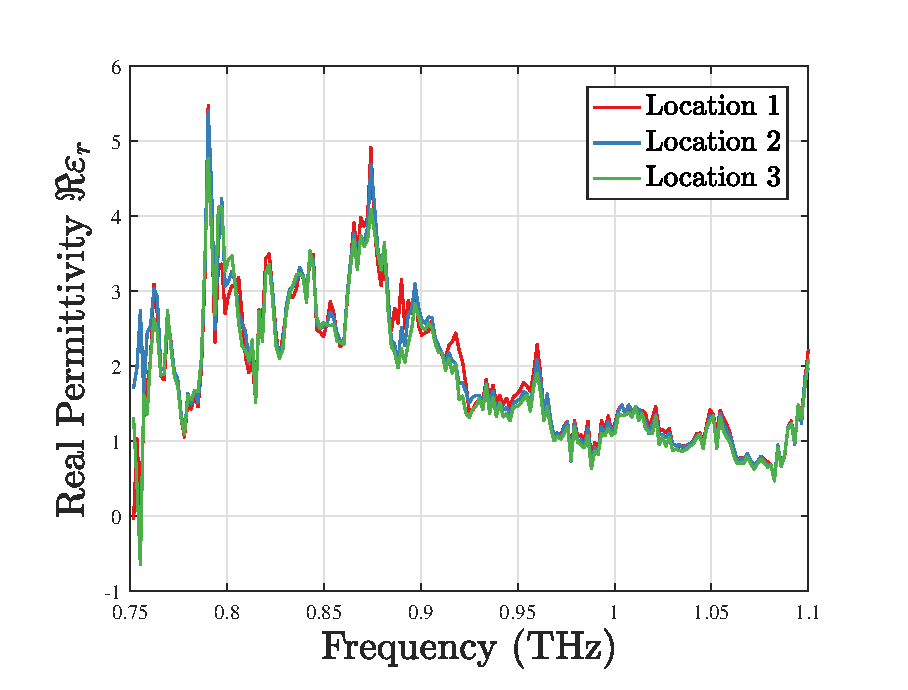
\includegraphics[width=0.48\linewidth]{coffee_day1R_revised.eps}
%		\label{fig:day1}
%	}
%	\hfill
%	\subfloat[Day 4]
%	{
%		\includegraphics[width=0.48\linewidth]{coffee_day4R_revised.eps}
%		\label{fig:day4}
%	}
%	\caption{Real part of permittivity of coffee leaves at three different locations taken on  day 1 and 4.}
%	\label{fig:coffee_days}
%\end{figure*}

In this paper, we present a novel, non-invasive approach to monitoring the WC of plant leaves using the scattering parameters of a THz pulse. Using a well-known material extraction algorithm, we computed permittivity from the scattering parameters for eight types of leaves, which we observed for four consecutive days. The WC was then gauged from the decrease in the permittivity as the days passed. This paper is an expansion and presents a detailed analysis of our earlier work \cite{Zahid2018}. 
%The significance of this paper lies in the simple, cost-effective technique and other advantages such as:
%\begin{figure*}[h!]
%	\centering
%	\includegraphics[trim={0.1cm 0cm 0cm 3cm}, clip,width=.55\linewidth]{RealSystem1.jpg}
%	\caption{Snapshot of System used for measurement of leaves. The sample is placed between the two corrugated waveguide}\label{fig:RealSystem1}
%\end{figure*}
%\begin{figure*}[h!]
%	\centering
%%	\includegraphics[trim={0cm 0cm 0cm 0cm}, clip,width=.45\linewidth]{setup8c.jpg}
%	\includegraphics[width=0.45\linewidth]{RealSystem1.jpg}
%	\includegraphics[width=0.45\linewidth]{leaves1.jpg}
%	\caption{{Snapshot of System used for measuring the transmission response of leaves. The sample is placed between the two corrugated waveguide.}
%	\label{fig:RealSystem1}
%	\caption{{Sample of Some fresh Plants leaves used for measurement purpose}\label{fig:leaves1}
%\end{figure*}
%
% \begin{figure*}[h!]
%	\centering
%	%\includegraphics[scale=0.26]{figs/fig1.png}
%	\includegraphics[width=0.45\linewidth]{TerahertzSensing1.jpg}
%	\caption{Internal Morphology of Fresh and Water stressed leaf using a Terahertz Sensing}
%	\label{fig:TerahertzSensing1}
%\end{figure*}
%
%\begin{figure*}
%  \begin{minipage}{0.48\linewidth}
%    \includegraphics[width=\linewidth ,height=6.5cm]{RealSystem1.jpg}
%    %\includegraphics[width=0.3\columnwidth]{treen2.jpg} % image of the n1
%    \captionof{figure}{Snapshot of System used for measuring the transmission response of leaves. The sample is placed between the two corrugated waveguide}\label{fig: RealSystem1}
%  \end{minipage}
%\hfill
%  \begin{minipage}{0.48\linewidth}
%	\includegraphics[width=\linewidth , height=6.5cm]{leaves1.jpg}
%	%\includegraphics[width=0.3\columnwidth]{treen1.jpg} % image of the n1
%	\captionof{figure}{Sample of Some fresh Plants leaves used for measurement purpose}\label{fig:leaves1}
%\end{minipage}
%\end{figure*}
%a) This paper proposes a unique technique to characterize and estimate WC of eight various leaves in terms of electromagnetic parameters at THz frequency range from 0.75 to 1.1 THz.
%b) The electromagnetic parameters are measured in simple, fast, and non-invasive manner using a terahertz material characterization kit. Moreover, The structural integrity and configuration of leaves were also considered by employing two Polytetrafluoroethylene (PTFE) caps which were fitted internally to the waveguide.
%% to provide uniform compression to soft samples, therefore avoiding any disturbances in the structural properties of the leaf samples.
%c) This paper establishes a notable correlation between electromagnetic parameters with WC in leaves i.e. an increment or decrement in WC status of leaves is evidently reflected in electromagnetic parameters at certain frequencies. 
The rest of the paper is structured as follows: Section \ref{sec:Experimental} describes the experimental setup followed by the material characterisation methods of plants leaves. {Section }\ref{sec:results}{ presents the measurement results and different parameters are discussed such as permittivity, the effect of weight and thickness, followed by a comparison of transmission response of all eight leaves between day 1 and 4}. Finally, conclusion is discussed in Section \ref{sec:conclusion}.
\section{Methods}\label{sec:Experimental}
%
\subsection{Experimental Setup}
%
%We used a THz Swissto12 Material Characterization (MCK) to obtain the scattering parameters of the plant leaves. The MCK was attached to a Virginia Diodes (VNA) extender WM-250 (WR1.0) operating in the frequency range of  0.75 to 1.1 THz. The VNA was powered by a Keysight Technologies PNA microwave network analyzer N5224A. 
{We used a Swissto12 material characterisation kit (MCK) operating in the THz frequency range to obtain the scattering parameters of the plant leaves. The MCK was attached to a Keysight Technologies N5224A microwave network analyser (NA), the frequency range of which was shifted in the THz frequency range via a Virginia Diode vector NA extender module WM-250 (WR 1.0), enabling operation in the frequency range of 0.75 to 1.1 THz with a resolution of 2 GHz. The MCK comprised of two conical waveguide horn transitions with further two sections of the low-loss corrugated waveguide. A small aperture between the two low-loss corrugated waveguides allows the material samples to be inserted into the system during the measurement. Moreover, each half of the MCK comprises a waveguide which transitions from a rectangular waveguide at one end to a corrugated circular waveguide at the other. Furthermore, one half of the MCK, is fixed, while the other half is movable (to easily accommodate the insertion of the sample to be measured)}. In order to avoid any structural damage while the leaf specimen was clamped in the MCK for observation, we used two PTFE caps that enabled a uniform compression of the samples as shown in Figure \ref{fig:setup8c} . Prior to the measurement, the setup was configured using the two-port short-open-load-thru (SOLT) calibration technique.

\begin{figure*}[t!]
	\centering
	%\includegraphics[trim={0cm 0cm 0cm 0cm}, clip,width=.65\linewidth]{setup8c.jpg}
	\includegraphics[trim={0cm 0cm 0cm 0cm}, clip,width=.65\linewidth]{setup8c.jpg}
	%	\includegraphics[width=.65\linewidth]{setup8c.jpg}
	\caption{Schematic representation of experimental setup used for measurement of leaf sample. The leaf sample is placed between the two PTFE caps fitted to waveguide}\label{fig:setup8c}
\end{figure*}

\begin{figure*}[t!]
	\centering
	\subfloat[Day 1]
	{
		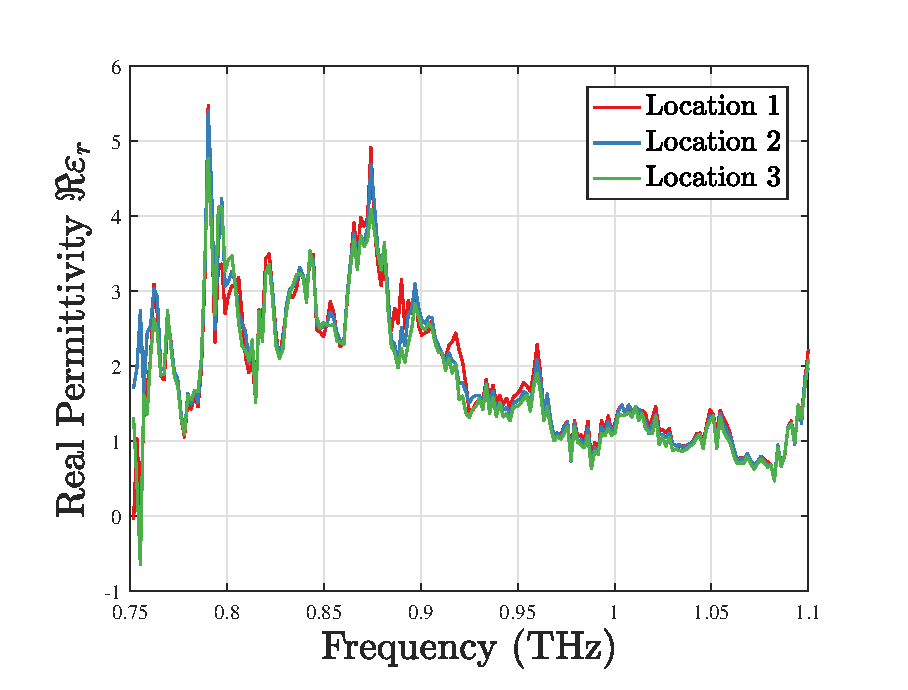
\includegraphics[width=0.48\linewidth]{coffee_day1R_revised.eps}
		\label{fig:day1}
	}
	\hfill
	\subfloat[Day 4]
	{
		\includegraphics[width=0.48\linewidth]{coffee_day4R_revised.eps}
		\label{fig:day4}
	}
	\caption{Real part of permittivity of coffee leaves at three different locations taken on days 1 and 4.}
	\label{fig:coffee_days}
\end{figure*}

\subsection{Sample Details}
%
Eight different kinds of pot herbs were used, namely coffee Arabica, aromatic coriander, basil, baby-leaf, pea-shoot, parsley, lamb lettuce, and baby spinach. The fresh leaves were detached from the plants and placed in the laboratory for four consecutive days. The environment temperature for the measurements of leaves was \SI{18 \pm .1}{\celsius}, and the humidity was between \SI{30 \pm 2}{\percent}. {In this study, the weight and thickness of leaves were determined for four consecutive days using a precision electronic scale and vernier calipers respectively.} The leaves' thickness and weight were measured every \SI{2}{\hour} during the natural evaporation of leaf moisture. We used a Vernier scale to measure the leaf thickness and this process was repeated to determine thicknesses at three different locations to ensure having similar all over the surface of a leaf, and found them in the threshold range of \SI{40}{\micro\m} to \SI{4}{\milli \metre}. The weight of leaf was measured using a digital kitchen scale with a least count of \SI{.1}{\mg}. All leaves were measured at three different locations and on every location, four various orientations were considered to investigate the behaviour of leaves. {From these observations, the purpose was mainly to determine any unevenness in the surface of leaves that may result in a change in the scattering response. For further illustration, Figure }\ref{fig:coffee_days} {shows the response of coffee leaf at three different locations which suggests that the orientation of leaf does not affect the measurements.}

\subsection{Material Characterisation of Plant Leaves}
%
%
The Nicholson-Ross-Weir (NRW) method \cite{nrw} is the most common technique in which the dielectric parameters $\varepsilon_r$ and $\mu_r$ of a planar material are extracted from a two-port vector NA measurement in which the transmission and reflection coefficients are obtained through the S-parameters. This method belongs to the category of frequency-by-frequency material extraction in which every point from the frequency sweep is used. In general, the NRW method generates both the complex permittivity $\varepsilon_r = \varepsilon_r'' - \j \varepsilon_r'$ and permeability, $\mu_r = \mu_r' - \j \mu_r''$ of the specimen under test. Here, we assume that the leaves are non-magnetic and compute only the permittivity.One of the intrinsic problems of the NRW method is the periodicity of the phase of the electromagnetic wave that leads to ambiguous results. This problem has been discussed at length in other works \cite{Weir1974,Baker1990,costa_electromagnetic_2017}. In order to rectify this, we follow the step-wise approach in which the phase ambiguity is removed by using the phase delay information from the previous frequency point \cite{Luukkonen2011}. In this paper, we consider a plant leaf as a planar slab of thickness $d$ which is positioned between two air-filled circular waveguides. With the help of an equivalent transmission line model, the reflection ($\Gamma$) and transmission ($T$) coefficients of a semi-infinite slab are expressed in terms of the measured s-parameters, $S_{11}$ and $S_{21}$ as \cite{boughriet_noniterative_1997},
%
\begin{align}
	\Gamma & = \chi \pm \sqrt{\chi^2 - 1}, & T & = \dfrac{S_{11} + S_{21} - \Gamma}{1 - \left( S_{11} + S_{21}\right) \Gamma}, 
	\label{eq:ref_tran_coefficients}
\end{align}
% 
where the intermediate variable $\chi$ is defined as $\left(S_{11}^2 - S_{21}^2 + 1\right)/{2 S_{11}}$. In the case of the slab having a finite thickness $d$, the transmission coefficient $T$ can described in terms of the propagation constant, $\gamma$ as, $T = \exp( - \gamma d)$,  which can subsequently be written in the Euler form as $|T| \exp(-j \phi)$ where $\phi$ denotes the phase term. The propagation constant is then determined using \cite{costa_electromagnetic_2017},
%
\begin{equation}
	\gamma = \frac{1}{d} \{ - \log(|T|) - \j \phi + \j 2 \pi n \} \, \mathrm{where}~ n \in \mathbb{Z}
	\label{eq:roots}
\end{equation}
%
which results in an infinite number of branches of the complex valued root due to the logarithmic function, demonstrated by the presence of the $2 \pi n$ term. The problem of selecting the proper branch is solved by the technique proposed in \cite{Luukkonen2011} in which at each frequency point, the phase delay information is recovered from the previous frequency point. If the phase difference, $\phi_i - \phi_{i-1} < \pi$, the method ensures the current branch is selected. The permittivity is then calculated by \cite{Kim2015},
% 
\begin{equation}
	\varepsilon_r = \frac{\gamma}{\gamma_0} \left[ \dfrac{1 - \Gamma}{1 + \Gamma} \right].
	\label{eq:permittivity}
\end{equation}
%
\section{{Results and Discussion}}
\label{sec:results}
%\begin{equation}
%\mathrm{n}=\frac{\ln T}{j k_{0} d}
%\end{equation}
%
%When the sample in our case leaves were placed in circular wave guide and as an electromagnetic wave propagates through plants leaves, initially transmission response for all leaves were measured overall power its power lessens due to the total power being spread over a wider surface area. Furthermore, it may suffer different types of attenuation or distortion due to absorption, scattering and refraction

In this paper, we aimed to determine the electromagnetic properties of leaves including permittivity, and physiological features such as weight and thickness that can affect the WC of leaves.  In addition, a strong correlation between the determined properties and WC of leaves was observed. Furthermore, the transmission response of all eight leaves were investigated for four consecutive days.

%{{\begin{figure}[h!]
%	\centering
%	%\includegraphics[scale=0.26]{figs/fig1.png}
%	%	\includegraphics[width=0.65\columnwidth]{TerahertzSensing3.jpg}
%	\includegraphics[width=0.55\textwidth]{TerahertzSensing5R.jpg}
%	\caption{Internal morphology of fresh and water stressed leaf using terahertz sensing.}
%	\label{fig:TerahertzSensing1}
%\end{figure}}}
%


% THREE BY THREE
%\begin{figure*}[t!]
%	\centering
%	\subfloat[Baby leaf]{\includegraphics[width=0.31\textwidth]{babyleaf_perm.eps}}
%	\label{fig:baby_eps}
%	\hfill
%	\subfloat[Basil leaf]{\includegraphics[width=0.31\textwidth]{basilleaf_perm.eps}}
%	\label{fig:basil_eps}
%	\hfill
%	\subfloat[Coffee Arabica]{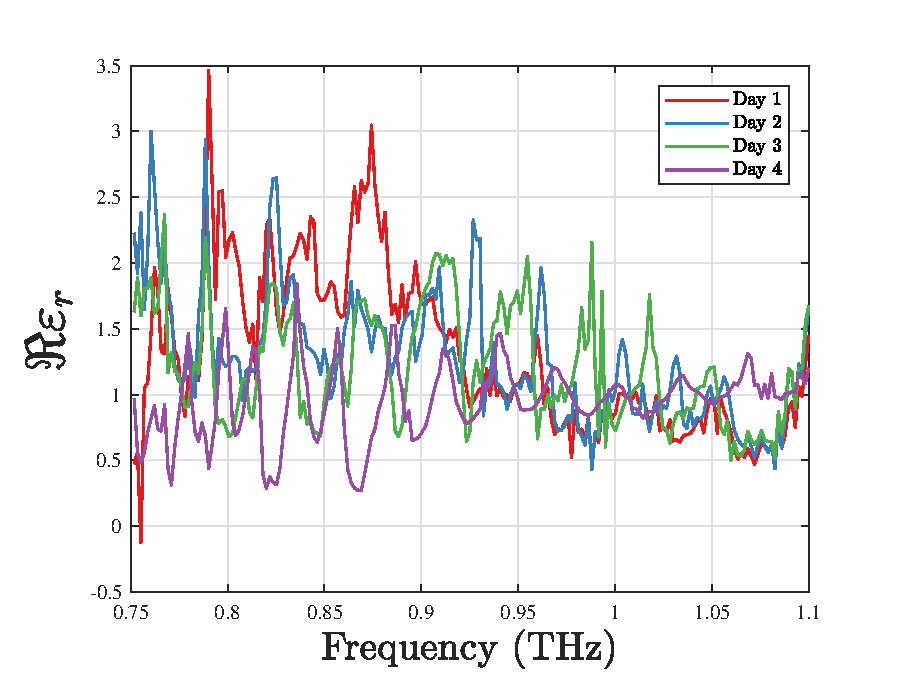
\includegraphics[width=0.31\textwidth]{coffeeleaf_perm.eps}}
%	\label{fig:coffee_eps}
%	\medskip
%	\subfloat[Aromatic Coriander]{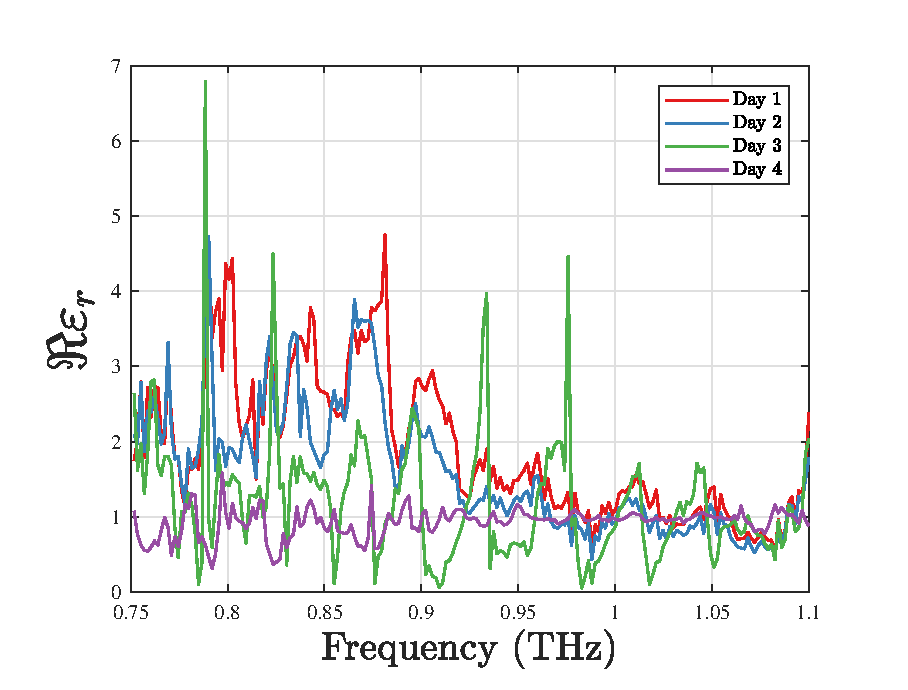
\includegraphics[width=0.31\textwidth]{corianderleaf_perm.eps}}
%	\label{fig:coriander_eps}
%	\hfill
%	\subfloat[Lamb Lettuce]{\includegraphics[width=0.31\textwidth]{lettuceleaf_perm.eps}}
%	\label{fig:lettuce_eps}
%	\hfill
%	\subfloat[Mint Leaf]{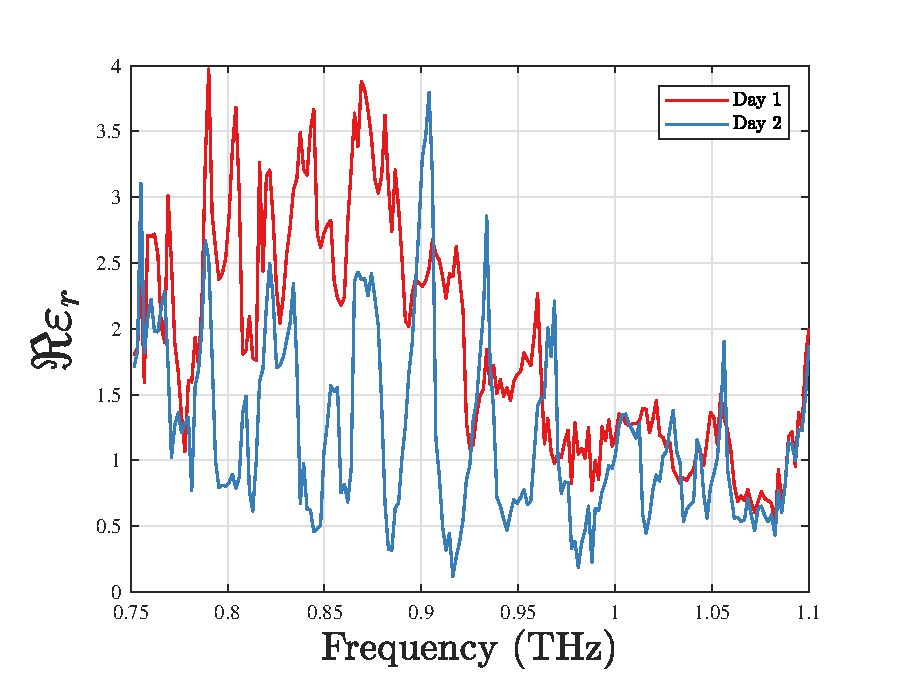
\includegraphics[width=0.31\textwidth]{mintleaf_perm.eps}}
%	\label{fig:mint_eps}
%	\medskip
%	\subfloat[Parsley]{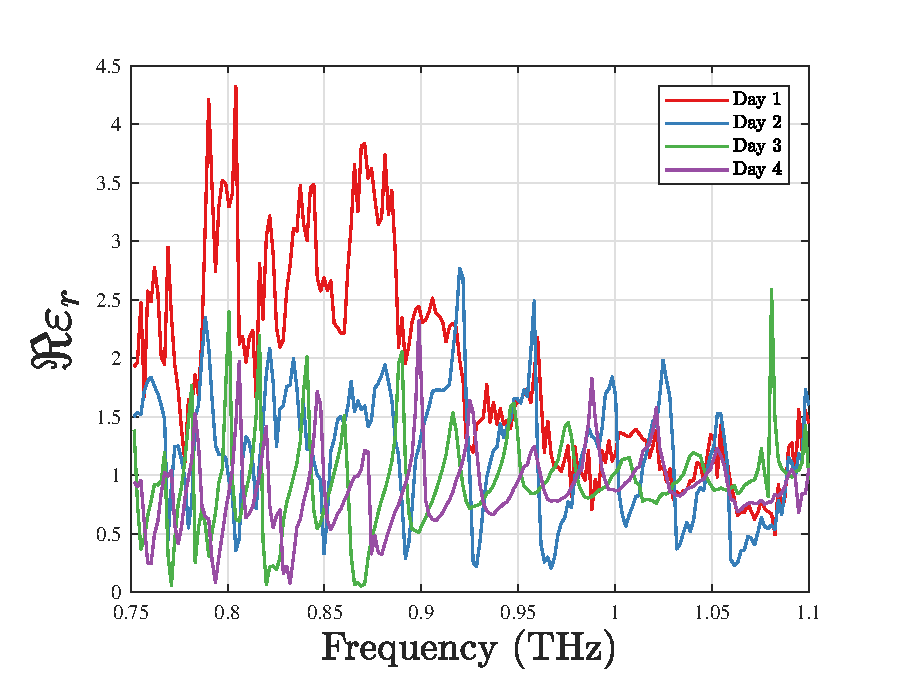
\includegraphics[width=0.31\textwidth]{parsleyleaf_perm.eps}}
%	\label{fig:parsley_eps}
%	\hfill
%	\subfloat[Peashoot]{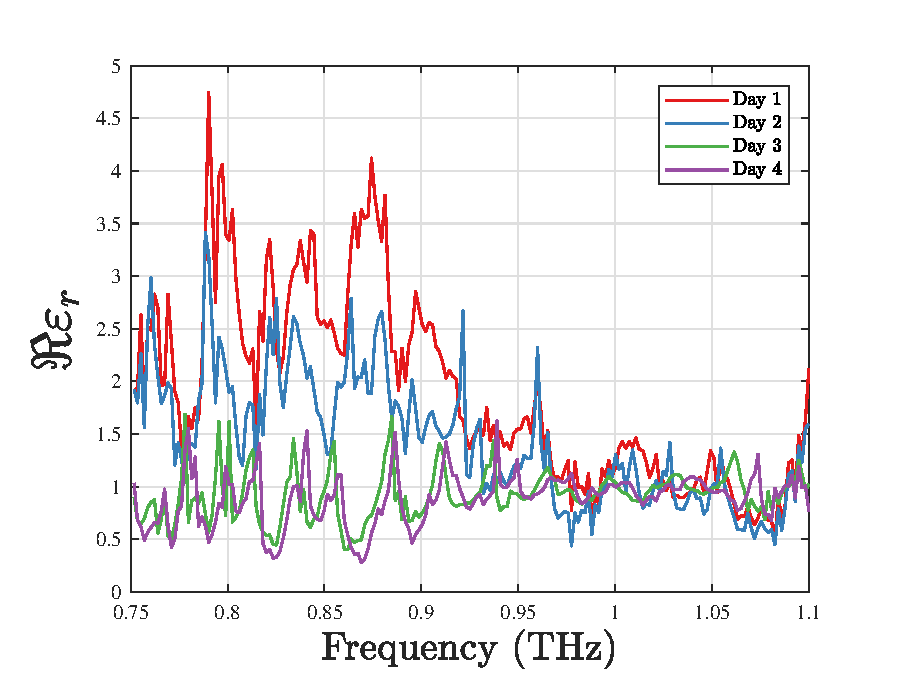
\includegraphics[width=0.31\textwidth]{peashootleaf_perm.eps}}
%	\label{fig:peashoot_eps}
%	\hfill
%	\subfloat[Baby Spinach]{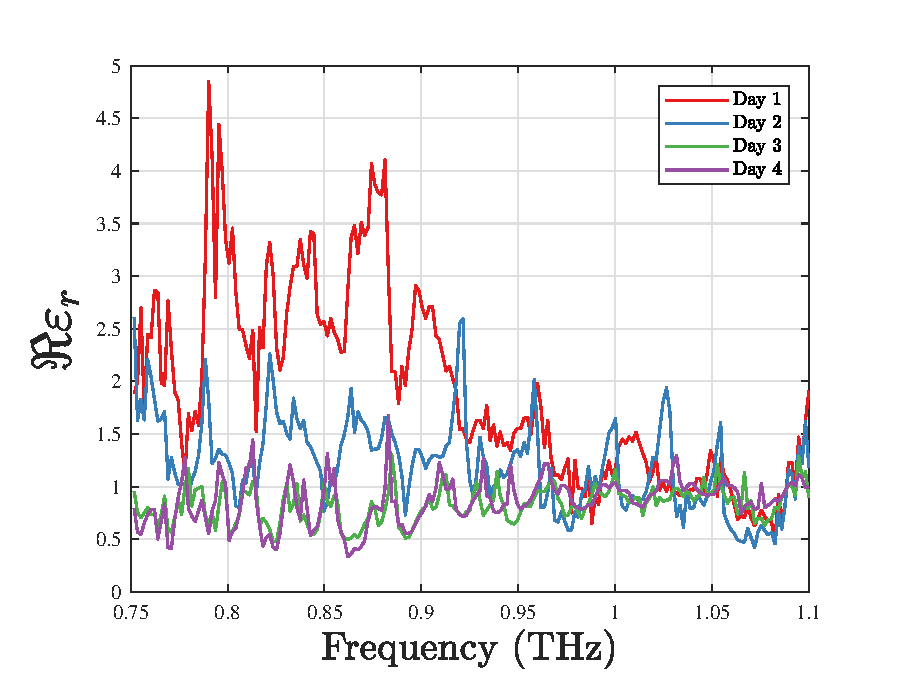
\includegraphics[width=0.32\textwidth]{spinachleaf_perm.eps}}
%	\label{fig:spinach_eps}
%	\caption{Real part of permittivity of all eight leaves measured on four consecutive days. Leaves become transparent to electromagnetic waves with the passage of days as seen by the decrease in the permittivity}
%	\label{fig:Permittivity_all_leaves}
%\end{figure*}



%\begin{figure*}[t!]
%	\centering
%	\subfloat[Baby leaf]{\includegraphics[width=0.32\textwidth]{/Used/baby_leaf_real_eps_all_days.tikz}}
%	\label{fig:baby_eps}
%	\hfill
%	\subfloat[Basil leaf]{\includegraphics[width=0.32\textwidth]{/Used/basil_leaf_real_eps_all_days.tikz}}
%	\label{fig:basil_eps}
%	\hfill
%	\subfloat[Coffee Arabica]{\includegraphics[width=0.32\textwidth]{/Used/coffee_leaf_real_eps_all_days.tikz}}
%	\label{fig:coffee_eps}
%	\medskip
%	\subfloat[Aromatic Coriander]{\includegraphics[width=0.32\textwidth]{/Used/coriander_leaf_real_eps_all_days.tikz}}
%	\label{fig:coriander_eps}
%	\hfill
%	\subfloat[Lamb Lettuce]{\includegraphics[width=0.32\textwidth]{/Used/lettuce_leaf_real_eps_all_days.tikz}}
%	\label{fig:lettuce_eps}
%	\hfill
%	\subfloat[Mint Leaf]{\includegraphics[width=0.32\textwidth]{/Used/mint_leaf_real_eps_all_days.tikz}}
%	\label{fig:mint_eps}
%	\medskip
%	\subfloat[Parsley]{\includegraphics[width=0.32\textwidth]{/Used/parsley_leaf_real_eps_all_days.tikz}}
%	\label{fig:parsley_eps}
%	\hfill
%	\subfloat[Peashoot]{\includegraphics[width=0.32\textwidth]{/Used/peashoot_leaf_real_eps_all_days.tikz}}
%	\label{fig:peashoot_eps}
%	\hfill
%	\subfloat[Baby Spinach]{\includegraphics[width=0.32\textwidth]{/Used/spinach_leaf_real_eps_all_days.tikz}}
%	\label{fig:spinach_eps}
%	\caption{Real part of permittivity of all eight leaves measured on four consecutive days. Leaves become transparent to electromagnetic waves with the passage of days as seen by the decrease in the permittivity}
%	\label{fig:Permittivity_all_leaves}
%\end{figure*}

\begin{figure*}[b!]
	\centering
	\subfloat[Baby leaf]{\includegraphics[width=0.49\textwidth]{babyleaf_perm_revised.eps}}
	\label{fig:baby_eps}
	\hfill
	\subfloat[Basil leaf]{\includegraphics[width=0.49\textwidth]{basilleaf_perm_revised.eps}}
	\label{fig:basil_eps}
	
	\subfloat[Coffee Arabica]{\includegraphics[width=0.49\textwidth]{coffeeleaf_perm_revised.eps}}
	\label{fig:coffee_eps}
	\hfill
	\subfloat[Aromatic Coriander]{\includegraphics[width=0.49\textwidth]{corianderleaf_perm_revised.eps}}
	\label{fig:coriander_eps}
\end{figure*}

\begin{figure*}[h!]
	\addtocounter{subfigure}{4}
	\centering
	\subfloat[e][Lamb Lettuce]{\includegraphics[width=0.49\textwidth]{lettuceleaf_perm_revised.eps}}
	\label{fig:lettuce_eps}
	\hfill
	\subfloat[Parsley]{\includegraphics[width=0.49\textwidth]{parsleyleaf_perm_revised.eps}}
	\label{fig:parsley_eps}
	
	\subfloat[Peashoot]{\includegraphics[width=0.49\textwidth]{peashootleaf_perm_revised.eps}}
	\label{fig:peashoot_eps}
	\hfill
	\subfloat[Baby Spinach]{\includegraphics[width=0.49\textwidth]{spinachleaf_perm_revised.eps}}
	\label{fig:spinach_eps}
	\caption{Real part of permittivity of all eight leaves measured on four consecutive days. Leaves become transparent to electromagnetic waves with the passage of days as seen by the decrease in the permittivity.}
	\label{fig:Permittivity_all_leaves}
\end{figure*}

\subsection{Permittivity of Leaves}
%
{The complex-valued permittivity of eight different types leaves were extracted from measurements taken from three various locations with different percentage of water content in them. Furthermore, on every location, measurements were recorded using four different orientations of the leaves to observe any anisotropic behaviour. Figure }\ref{fig:day1}{ shows that for a coffee Arabica leaf, neither the location, nor the leaf orientation had any effect on the real part of permittivity on day 1. However, the effect of location was notable on the day 4 as shown in Figure }\ref{fig:day4}{. We believe that the drastic decrease in the leaf thickness is responsible for this behaviour.}

%It is also perceived from the  Fig. \ref{fig:Permittivity_all_leaves} that with every passing day, permittivity seemed to be decreasing due to loss of moisture cells or \ac{wc} in leaves%$$ $$$$$$$$$$$$$$$$$$$$$$$$$$$$$$$$44

%\begin{figure}[t!]
%	\centering
%	{\includegraphics[width=0.48\textwidth]{permittivity_water.eps}}
%	%	\caption{Correlation of permittivity with loss of \ac{wc} in leaves over four days.}
%	\caption{Correlation of permittivity with loss of WC in leaves.}
%	\label{fig:correlation_perm}
%\end{figure}

\begin{figure}[t!]
	\centering
	\includegraphics[width=0.48\textwidth]{perm_with_water_content2.eps}
	%	\caption{Correlation of permittivity with loss of \ac{wc} in leaves over four days.}
	\caption{{Correlation of permittivity with loss of WC in leaves.}}
	\label{fig:correlation_perm}
\end{figure}
% 
{Similar patterns were observed for other types of leaves as well.} Figure \ref{fig:Permittivity_all_leaves} {shows} the real part of the permittivity for all the leaves measured on four consecutive days. It {is} significant to observe that all the leaves revealed the highest permittivity on day 1 when the WC in fresh leaves {was the highest}, and as the days progressed, permittivity showed a decrement when leaves became water stressed. Hence, dielectric parameter measurements differed significantly on {days} 1 and 4 for fresh, and water-stressed leaves. From these observations, it also showed a clear correlation between the permittivity and WC of leaves, i.e. fresh leaves with a higher amount of WC would have a high permittivity and vice versa. From Figure \ref{fig:correlation_perm}, it {is evident that the real part of }permittivity {shows} a strong decaying correlation with WC. As observed in Figure \ref{fig:Permittivity_all_leaves}, various leaves also showed {distinct decreasing responses from each other, attributed to different lead composition and structure. In an another study, we have shown that the real part of permittivity can be used to classify leaves, that are described here with an accuracy of 98.2 \%.}
% It can be validated with the obtained Fig. \ref{fig:Permittivity_all_leaves} where strong peaks or deviations were observed on day 1 and 2 by all leaves between a frequency range of 0.75 to 0.95 THz, and then the leaves exhibited a decay in peaks as the days passed, specifically on day 4 between a frequency range of 1 to 1.1 THz.In conclusion, increasing or decreasing \ac{wc} in leaves over the course of four days showed a high significantly correlations with permittivity of leaves.that after frequency range of 0.75 THz to 0.9 THz or up to 0.95 for some leaves, not very sharp variations or high peaks were occurred leading to decrement in permittivity. However, by comparing the leaves permittivity of day 1 with day 4, day 1 appeared to be is still high than at day4 despite of individually trends to be in decreasing pattern. It shows \ac{wc} in fresh leaves at leaves permittivity of day 1 with day 4, day 1 appeared to be is still high than at day4 despite of individually trends to be in decreasing pattern. It shows \ac{wc} in fresh leaves at day1 is comparatively more in volumes than leaves that are dried out resulting a less \ac{wc} in them. With every passing days, leaves were noticed to be getting highly drought and as expected, believed to have less water molecules than day1.The focus of research under this section is to establish an understanding of dielectric properties of various plant leaves and observed their reactions in different conditions. It was realized that because of various, sizes, shapes and orientations of different plant leaves, permittivity would be affected. The study was focused mainly on eight leaves, coffee, basil, coriander, lettuce, baby-leaf, pea-shoot, mint, parsley and spinach. Therefore, it can be concluded that the structural characteristics of vegetation also have a certain effect on the real parts of complex permittivity and there seemed to be a mutual correlation between them.
% 
%{{}}\subsection{Refractive Index of Leaves}
%In this section, the refractive indices for all the leaves with variance level of WC were computed. It was examined that different leaves performed individually due to the internal characteristics of leaves and the amount of WC presence in the leaves at the time of measurement. Likewise, the same pattern was repeated to determine the refractive index of all leaves for four days. For some leaves as shown in Figure \ref{fig:N_all_leaves}, a very robust and strong abnormal dispersion was perceived, which was clearly attributed to the presence of large WC.}}
% 
% 
%Whereas in others, standard scattering was noticed which again evidently showed a characteristic of those leaves followed by the presence of WC to a least.
%{{}}There is another significant optical parameter which can exploit the different characteristics of plant leaves and provide very meaningful and useful information about WC in leaves.}}
% 
%In this section, we present the refractive indices for all the leaves that were computed by taking the real part of the square-root of the complex permittivity.It was examined that different leaves performed individually due to the internal characteristics of leaves and the amount of \ac{wc} presence in the leaves at the time of measurement. Likewise, set locations on all leaves.
%It was examined that different leaves performed individually due to the internal characteristics of leaves and the amount of \ac{wc} presence in the leaves at the time of measurement. Likewise, previously mentioned, same pattern was repeated to determine the refractive index for four days for all leaves. For some leaves as shown in Fig \ref{fig:N_all_leaves}, it was perceived a very robust and strong abnormal dispersion which was clearly attributed to the presence of large water content in those leaves. Whereas in others, standard scattering was noticed which again evidently showed a characteristic of those leaves followed by the presence of \ac{wc} to a least.\\\textbf
%\subsubsection{Relation of Refractive Index with WC}
%From Fig \ref{fig:Refractive index}, it was discovered that refractive index exhibited a decrement correlation with \ac{wc} as the days passed. This exponential decay in electromagnetic parameter was attributed to waster moisture in leaves which had been dehydrating from day 1 to 4. From Fig \ref{fig:Refractive index}, it was also noticed that As observed in \ref{fig:permittivity}, various leaves also showed distinctive decrement responses from each other, also attributing to have physiological and biological process growth. In this process, specific values of permittivity were investigated with water loss of leaves from day 1 to 4.
% 
%This parameter has a clear correlation with the absorption of water molecules in leaves, i.e., larger the absorption of water molecular, higher and strong deviation is expected as an outcome response of leaves. In other words, attenuation would be higher for the presence of large volumetric presence of \ac{wc} in leaves. In this study, this was validated when the leaves were tested for refractive index on first day when the leaves were fresh, a strong eccentric was obtained indicating the water status in leaves to large extent. The same leaves were tested on following days, and degree of attenuation was reduced, and low peaks were attained demonstrating the water molecules had been evaporated with the passing time.
% 
% 
%{{}}\begin{figure*}[bh!]
%	\centering
%	\subfloat[Baby leaf]{\includegraphics[width=0.49\textwidth]{babyleaf_ref_revised.eps}}
%	\label{fig:baby_n}
%	\hfill
%	\subfloat[Basil leaf]{\includegraphics[width=0.49\textwidth]{basilleaf_ref_revised.eps}}
%	\label{fig:basil_n}
%	
%	\subfloat[Coffee Arabica]{\includegraphics[width=0.49\textwidth]{coffeeleaf_ref_revised.eps}}
%	\label{fig:coffee_n}
%	\hfill
%	\subfloat[Aromatic Coriander]{\includegraphics[width=0.49\textwidth]{corianderleaf_ref_revised.eps}}
%	\label{fig:coriander_n}
%\end{figure*}
%\begin{figure*}[th!]
%	\addtocounter{subfigure}{4}
%	\centering
%	\subfloat[Lamb Lettuce]{\includegraphics[width=0.49\textwidth]{lettuceleaf_ref_revised.eps}}
%	\label{fig:lettuce_n}
%	\hfill
%	%	\subfloat[Mint Leaf]{\includegraphics[width=0.49\textwidth]{mintleaf_ref.eps}}
%	%	\label{fig:mint_n}
%	\subfloat[Parsley]{\includegraphics[width=0.49\textwidth]{parsleyleaf_ref_revised.eps}}
%	\label{fig:parsley_n}
%	
%	\subfloat[Peashoot]{\includegraphics[width=0.49\textwidth]{peashootleaf_ref_revised.eps}}
%	\label{fig:peashoot_n}
%	\hfill
%	\subfloat[Baby Spinach]{\includegraphics[width=0.49\textwidth]{spinachleaf_ref_revised.eps}}
%	\label{fig:spinach_n}
%	\caption{Real part of refractive index of all the eight leaves measured on four consecutive days.}
%	\label{fig:N_all_leaves}
%\end{figure*}}}
% 
% 
\subsection{{Estimating Leaf Water Content}}
% The water status of plant leaves is directly related to the physiological growth process and assessing the drought stress of leaves. Therefore, it is an essential and useful information to monitor the \ac{wc} on a frequent basis to avoid severe scarcity in leaves.
%In this study, the weight and thickness of leaves were determined for consecutively four days using precision tool electronic scale and Vernier calipers respectively. Referring to the weights of leaves, initially on the first day, the time duration between the two weight measurements were maintained between two to three hours. On the second day, this was extended to four hours and finally, on the third and fourth days, it was increased to 6 hours. Intriguingly, it was markedly noticed that there was significant decrement in the weights of some leaves as shown in Fig. \ref{fig:weight} on day 1, i.e. basil, baby leaf and pea-shoot, whereas, other leaves displayed a slow decrement in weight loss of leaves as days progressed. This clearly indicated that \ac{wc} in leaves evaporated more rapidly on the day 1 and 2 comparing to day 3 and 4, creating more air cavity in the leaves. To assess the variation of leaf \ac{wc} during the leaf water evaporation process, the measurements were translated into \ac{wc} using \cite{Nie2017,Cao2015},
In this study, WC in leaves was observed by determining the physical parameters such as weight and thickness. Referring to the weight of leaves, initially on the first day, the time duration between the two weight measurements were maintained from two to three hours. On the second day, this was extended to four hours and finally, on the third and fourth day, it was increased to 6 hours. It was noted that there was significant {decrease} in the weights of some leaves as shown in Figure \ref{fig:measurements} on day 1, i.e. basil, baby leaf and pea shoot, whereas, other leaves displayed a slow decreasing trend in weight loss of leaves as days progressed.
\begin{figure*}[h!]
	\centering
	\subfloat[Weight]
	{
		\includegraphics[width=0.485\textwidth]{water_content.eps}
		\label{fig:weight}
	}
	\hfill
	\subfloat[Thickness]
	{
		\includegraphics[width=0.485\textwidth]{thickness.eps}
		\label{fig:thickness}
	}
	\caption{Change in the physical properties of leaves with time.}
	\label{fig:measurements}
\end{figure*}
%\begin{figure*}[h!]
%	\centering
%	\subfloat[Weight]
%	{
%		\includegraphics[width=0.45\textwidth]{water_content.eps}
%		\label{fig:weight}
%	}
%	\hfill
%	\subfloat[Thickness]
%	{
%		\includegraphics[width=0.45\textwidth]{thickness.eps}
%		\label{fig:thickness}
%	}
%	\caption{Change in the physical properties of leaves with time.}
%	\label{fig:measurements}
%\end{figure*}
%
%\begin{figure*}[h!]
%	\centering
%	\subfloat[Day 1]{\includegraphics[width=0.45\textwidth]{Pathloss_day1.eps}}
%	\hfill
%	\label{fig:pathloss_day1}
%	\subfloat[Day 4]{\includegraphics[width=0.45\textwidth]{Pathloss_day4.eps}}
%	\label{fig:pathloss_day4}
%	%  \caption{Path loss in all the leaves on days 1 and 4.}
%	\caption{Transmission response of leaves on day 1 and 4.}
%	\label{fig:pathloss}
%\end{figure*}
This clearly indicated that the moisture in leaves evaporated more rapidly on the day 1 and 2 compared to day 3 and 4, thereby creating more air cavities in the leaves. To assess the variation of leaf WC during the leaf's water evaporation process, the measurements were translated into WC using \cite{Nie2017,Cao2015},
\begin{equation}
	WC = \frac{W_{\mathrm{time}} - W_{\mathrm{dry}}}{W_{\mathrm{fresh}}} \times 100%
	\label{eq:WC}
\end{equation}
where $W_{\mathrm{fresh}}$ is the weight of the fresh leaf, $W_{\mathrm{time}}$ is the weight of a leaf measured over time and $W_{\mathrm{dry}}$ is the weight of a dry leaf. In the beginning, the WC loss observed between the two hours on day 1 was found in the range of 5\% to 22\%. At the end of the investigation on day 4, this loss was increased during the natural evaporation of leaf moisture and was established in the range of 83.12\% to 99.33\%.
%fresh measurements and day 4 dry measurements of all leaves including baby, basil, coriander, coffee, lamb lettuce, parsley, pea-shoot, spinach were 91.19\%, 95.80\%, 93.00\%, 91.72\%, 97.36\%, 93.16\%, 86.23\%, 99.10\%, 99.33\% respectively.
The obtained percentages loss of WC can be validated with Figure \ref{fig:weight}. Considering this discussion, it also showed a significant correlation with the real part of the permittivity which was the highest on the first day when the weight of leaves was considerably high compared with the fourth day as shown in Figure \ref{fig:Permittivity_all_leaves}.
%\begin{figure*}[h!]
%	\centering
%	\subfloat[Day 1]{\includegraphics[width=0.42\textwidth]{Pathloss_day1.eps}}
%	\hfill
%	\label{fig:pathloss_day1}
%	\subfloat[Day 4]{\includegraphics[width=0.42\textwidth]{Pathloss_day4.eps}}
%	\label{fig:pathloss_day4}
%	%  \caption{Path loss in all the leaves on days 1 and 4.}
%	\caption{Transmission response of leaves on day 1 and 4.}
%	\label{fig:pathloss}
%\end{figure*}
%\begin{figure*}[t!]
%  \centering
%  \subfloat[Day 1]{\includegraphics[width=0.45\textwidth]{/Used/Pathloss_day1.tikz}}
%  \hfill
%  \label{fig:pathloss_day1}
%  \subfloat[Day 4]{\includegraphics[width=0.45\textwidth]{/Used/Pathloss_day4.tikz}}
%  \label{fig:pathloss_day4}
%  %  \caption{Path loss in all the leaves on days 1 and 4.}
%  \caption{Path-loss Response of leaves considering the effect of Water Content in leaves on day 1 and day 4.}
%  \label{fig:pathloss}
%\end{figure*}
%Furthermore,along with loss in weight of leaves due to decrement in water status in leaves,Furthermore, another characteristic that could affect the loss in \ac{wc} is the thickness of leaves.
%The thickness of all the leaves was carefully determined avoiding any excess pressure to the samples, that would cause disturbances in the morphological structure of leaves, therefore changing the dielectric properties of the samples as a result. It can be clearly illustrated from the Fig. \ref{fig:thickness} that the thickness of leaves was considerably higher on day 1, attributing a hefty presence of \ac{wc} in fresh leaves compared to day 4 when the leaves were dried out. From this significant and meaningful observation, it is concluded that dehydration of water contents in leaves with passing days affected the thicknesses to substantial degree. On day 4, some leaves stayed invariant or slight changes occurred in the thickness of leaves i.e. coriander and spinach as shown in Fig. \ref{fig:weight}. These transformations in the thickness of leaves evidently show that \ac{wc} in coriander and spinach leaves had been evaporated to the maximum on day 4 and no further variations could be observed in thickness of leaves.
The thickness of all the leaves was carefully determined to avoid any excess pressure to the samples, that would cause disturbances in the morphological structure of the leaves, changing the dielectric properties of the samples as a result. As seen in Figure \ref{fig:thickness}, the thickness of leaves was considerably higher on day 1, implying a greater WC in fresh leaves compared to day 4 when mostly, all leaves were dried out. From this significant and meaningful observation, it was concluded that dehydration of water contents in leaves with passing days affected the thicknesses to a substantial degree. On day 4, some leaves stayed invariant or slight changes occurred in the thickness of leaves i.e. coriander and spinach as shown in Figure \ref{fig:weight}. These transformations in the thickness of leaves evidently showed that WC in coriander and spinach leaves had evaporated to the maximum on day 4 and no further variations could be observed in thickness of leaves.
\subsection{Evaluation of Leaf Transmission Response}
%
%When \ac{thz} waves propagated through various leaves on day 1 and 4, there were transmission loss occurring in the leaves. Interestingly, the loss appeared different for each leaf, possibly attributed to the different chemical compositions. From the Fig. \ref{fig:pathloss}, on day 1, it was noticed that loss occurred was considerably high, indicating a high \ac{wc} in the leaves. Correspondingly, upon a close analysis, the path-loss response of leaves on day 4 compared to day 1 came out substantially low as shown in Fig. \ref{fig:pathloss}, because leaves were dried out, showing minimum signs of \ac{wc} in the leaf tissues. Hence, the path-loss has a clear relation with volumetric amount of \ac{wc} in leaves, even exhibited to similar environmental conditions.
In this section, transmission responses of all leaves were observed on day 1 and 4 as shown in Figure \ref{fig:pathloss}. It was noticed that on day 1, attenuations of all leaves were substantially high due to the presence of higher WC in tissues of leaves, which resulted in a higher absorption and lower transmission response. Moreover, on day 4, a substantial degree of increment in transmission response was observed as WC in leaves had evaporated to large extent, which resulted in a decrement of weight and thickness of leaves and eventually, less absorption occurred at this time. Figure \ref{fig:pathloss} exhibited a strong correlation of transmission response with WC, weight and thickness of leaves. Baby-leaf exhibited a lower transmission response on day 1 compared to others, reflecting a higher presence of WC in leaf, which resulted in higher absorption. Contrarily, parsley displayed an increment in transmission response due to the presence of less WC in the leaf and,hence, producing low absorption compared to other leaves.
% , weight and thickness, as well as the surface roughness of leaves occurred due to the evaporation of water molecules over the course of four days and can be validated with the  path-loss \ref{fig:pathloss} and \ref{fig:pathloss}, and weight and thickness of leaves fig\ref{fig:weight} and \ref{fig:thickness}. Moreover, distinct behavior of path-loss response over the course of four days can also affect characteristics of leaves at cellular level.
%
%By comparing \ref{fig:pathloss_day1} and \ref{fig:pathloss_day4}, it can be stated that difference in path-loss is also attributed to the difference in morphological and physiological characteristics of leaves occurred over the four days and depends on water content presence in tissue of leaves even when exposed to the same environmental determinants. Moreover,

%
%\begin{figure*}[t!]
%  \centering
%  \subfloat[Day 1]{\includegraphics[width=0.45\textwidth]{/Used/Pathloss_day1.tikz}}
%  \hfill
%  \label{fig:pathloss_day1}
%  \subfloat[Day 4]{\includegraphics[width=0.45\textwidth]{/Used/Pathloss_day4.tikz}}
%  \label{fig:pathloss_day4}
%  \caption{Path loss in all the leaves on days 1 and 4.}
%  \label{fig:pathloss}
%\end{figure*}
%

%%In addition, path-loss has a clear correlation with the absorption of water molecules in leaves, weight and thickness of leaves.
%If the absorption or attenuation in transmission response leaves is high, it reveals the meaningful information that it could be either due to the surface roughness of leaves, \ac{wc}, weight and thickness of leaves or the propagation properties during the process of their growth. Comparing the Figs. \ref{fig:pathloss_day1} and \ref{fig:pathloss_day4}, it can be seen that path-loss response in day 4 than in day1, which clearly indicates that over the course of four-day period, there is significant change in characteristics at cellular level in leaves.\\
%
\begin{figure*}[h!]
	\centering
	\subfloat[Day 1]{\includegraphics[width=0.49\textwidth]{Pathloss_day1.eps}}
	\hfill
	\label{fig:pathloss_day1}
	\subfloat[Day 4]{\includegraphics[width=0.49\textwidth]{Pathloss_day4.eps}}
	\label{fig:pathloss_day4}
	%  \caption{Path loss in all the leaves on days 1 and 4.}
	\caption{Transmission response of leaves on first and fourth days.}
	\label{fig:pathloss}
\end{figure*}

\section{Conclusion}
\label{sec:conclusion}
%
%In this paper, a novel, non-invasive technique of characterizing the water content, and in turn the health of plant leaves was proposed using terahertz waves. The electromagnetic properties of eight types of leaves were determined for four consecutive days through the measured scattering parameters. The weight and thickness of the leaves were also recorded at the same time. We observed that the leaves became increasingly transparent to the terahertz waves through the course of the four day experiment, as seen by the peaks of the permittivity as well as the refractive index of the leaves. With the help of weight and thickness measurements, we deduce that the water content of the plant leaves is strongly correlated to the transmission response.

In this paper, a novel, non-invasive technique of characterising the water content, and in turn the health of plant leaves was proposed using THz waves. The electromagnetic properties of eight types of leaves were determined for four consecutive days through the measured scattering parameters. The weight and thickness of the leaves were also recorded at the same time. We observed that the leaves became increasingly transparent to the terahertz waves through the course of four days experiment, {as seen by the peaks in the real part of permittivity}. Similar decaying trends were observed in the peak values of the real part of the extracted relative permittivity as the decreasing weight due to loss of water content. {The significance of this paper lies in the simple, cost-effective technique and other advantages such as: a) This paper proposes a unique technique to characterise and estimate WC of eight various leaves in terms of electromagnetic parameters at THz frequency range from 0.75 to 1.1 THz.
b) The electromagnetic parameters are measured in simple, fast, and non-invasive manner using a terahertz material characterisation kit. Moreover, The structural integrity and configuration of leaves were also considered by employing two polytetrafluoroethylene (PTFE) caps which were fitted internally to the waveguide.
% to provide uniform compression to soft samples, therefore avoiding any disturbances in the structural properties of the leaf samples.
c) This paper establishes a notable correlation between electromagnetic parameters with WC in leaves i.e. change in the WC of leaves is reflected in the electromagnetic parameters at certain frequencies.} In the age of a climate change driven water conservation, the proposed scheme can be used to design efficient irrigation systems on-site without any need to remove the leaves from plants. 
%The significance of this paper lies in employing this novel technique for the first time to obtain terahertz characterizations and the water content of eight leaves in the simple, fast and reliable way. 

%\section{Section title}
%\label{sec:1}
%Text with citations \cite{RefB} and \cite{RefJ}.
%\subsection{Subsection title}
%\label{sec:2}
%as required. Don't forget to give each section
%and subsection a unique label (see Sect.~\ref{sec:1}).
%\paragraph{Paragraph headings} Use paragraph headings as needed.
%\begin{equation}
%a^2+b^2=c^2
%\end{equation}

% For one-column wide figures use
%\begin{figure}
%% Use the relevant command to insert your figure file.
%% For example, with the graphicx package use
%  \includegraphics{example.eps}
%% figure caption is below the figure
%\caption{Please write your figure caption here}
%\label{fig:1}       % Give a unique label
%\end{figure}
%
% For two-column wide figures use
%\begin{figure*}
%% Use the relevant command to insert your figure file.
%% For example, with the graphicx package use
%  \includegraphics[width=0.75\textwidth]{example.eps}
%% figure caption is below the figure
%\caption{Please write your figure caption here}
%\label{fig:2}       % Give a unique label
%\end{figure*}
%
% For tables use
%\begin{table}
%% table caption is above the table
%\caption{Please write your table caption here}
%\label{tab:1}       % Give a unique label
%% For LaTeX tables use
%\begin{tabular}{lll}
%ine\noalign{\smallskip}
%first & second & third  \\
%\noalign{\smallskip}ine\noalign{\smallskip}
%number & number & number \\
%number & number & number \\
%\noalign{\smallskip}ine
%\end{tabular}
%\end{table}


%\begin{acknowledgement}
%\\
%Adnan Zahid is funded by EPSRC doctoral training programme. Sincere thanks to CSI members, School of Electronic and Nanoscale engineering department, University of Glasgow for their useful and valuable suggestions.
%\end{acknowledgement}



\section*{Acknowledgment}
Adnan Zahid is funded by EPSRC doctoral training programme. Sincere thanks to CSI members, School of Electronic and Nanoscale engineering department, University of Glasgow for their useful and valuable suggestions.

%%%%%%%%%%%%%%%%%%%%%%%%%%%%%%%%%%%%%%%%%%%%%%%%%%%%%
%\section{Results}
%
%This section may be divided by subheadings. It should provide a concise and precise description of the experimental results, their interpretation as well as the experimental conclusions that can be drawn.
%\begin{quote}
%This section may be divided by subheadings. It should provide a concise and precise description of the experimental results, their interpretation as well as the experimental conclusions that can be drawn.
%\end{quote}
%
%%%%%%%%%%%%%%%%%%%%%%%%%%%%%%%%%%%%%%%%%%%
%\subsection{Subsection}
%\unskip
%\subsubsection{Subsubsection}
%
%Bulleted lists look like this:
%\begin{itemize}[leftmargin=*,labelsep=5.8mm]
%\item	First bullet
%\item	Second bullet
%\item	Third bullet
%\end{itemize}
%
%Numbered lists can be added as follows:
%\begin{enumerate}[leftmargin=*,labelsep=4.9mm]
%\item	First item
%\item	Second item
%\item	Third item
%\end{enumerate}
%
%The text continues here.
%
%\subsection{Figures, Tables and Schemes}
%
%All figures and tables should be cited in the main text as Figure 1, Table 1, etc.
%
%\begin{figure}[H]
%\centering
%\includegraphics[width=2 cm]{Definitions/logo-mdpi}
%\caption{This is a figure, Schemes follow the same formatting. If there are multiple panels, they should be listed as: (\textbf{a}) Description of what is contained in the first panel. (\textbf{b}) Description of what is contained in the second panel. Figures should be placed in the main text near to the first time they are cited. A caption on a single line should be centered.}
%\end{figure}
%
%Text
%
%Text
%
%\begin{table}[H]
%\caption{This is a table caption. Tables should be placed in the main text near to the first time they are cited.}
%\centering
%%% \tablesize{} %% You can specify the fontsize here, e.g., \tablesize{\footnotesize}. If commented out \small will be used.
%\begin{tabular}{ccc}
%\toprule
%\textbf{Title 1}	& \textbf{Title 2}	& \textbf{Title 3}\\
%\midrule
%entry 1		& data			& data\\
%entry 2		& data			& data\\
%\bottomrule
%\end{tabular}
%\end{table}
%
%Text
%
%Text
%
%%\begin{listing}[H]
%%\caption{Title of the listing}
%%\rule{\textwidth}{1pt}
%%\raggedright Text of the listing. In font size footnotesize, small, or normalsize. Preferred format: left aligned and single spaced. Preferred border format: top border line and bottom border line.
%%\rule{\textwidth}{1pt}
%%\end{listing}
%
%
%\subsection{Formatting of Mathematical Components}
%
%This is an example of an equation:
%
%\begin{equation}
%a + b = c
%\end{equation}
%%% If the documentclass option "submit" is chosen, please insert a blank line before and after any math environment (equation and eqnarray environments). This ensures correct linenumbering. The blank line should be removed when the documentclass option is changed to "accept" because the text following an equation should not be a new paragraph.
%
%Please punctuate equations as regular text. Theorem-type environments (including propositions, lemmas, corollaries etc.) can be formatted as follows:
%%% Example of a theorem:
%\begin{Theorem}
%Example text of a theorem.
%\end{Theorem}
%
%The text continues here. Proofs must be formatted as follows:
%
%%% Example of a proof:
%\begin{proof}[Proof of Theorem 1]
%Text of the proof. Note that the phrase `of Theorem 1' is optional if it is clear which theorem is being referred to.
%\end{proof}
%The text continues here.
%
%%%%%%%%%%%%%%%%%%%%%%%%%%%%%%%%%%%%%%%%%%%
%\section{Discussion}
%
%Authors should discuss the results and how they can be interpreted in perspective of previous studies and of the working hypotheses. The findings and their implications should be discussed in the broadest context possible. Future research directions may also be highlighted.
%
%%%%%%%%%%%%%%%%%%%%%%%%%%%%%%%%%%%%%%%%%%%
%\section{Materials and Methods}
%
%Materials and Methods should be described with sufficient details to allow others to replicate and build on published results. Please note that publication of your manuscript implicates that you must make all materials, data, computer code, and protocols associated with the publication available to readers. Please disclose at the submission stage any restrictions on the availability of materials or information. New methods and protocols should be described in detail while well-established methods can be briefly described and appropriately cited.
%
%Research manuscripts reporting large datasets that are deposited in a publicly available database should specify where the data have been deposited and provide the relevant accession numbers. If the accession numbers have not yet been obtained at the time of submission, please state that they will be provided during review. They must be provided prior to publication.
%
%Interventionary studies involving animals or humans, and other studies require ethical approval must list the authority that provided approval and the corresponding ethical approval code.
%
%%%%%%%%%%%%%%%%%%%%%%%%%%%%%%%%%%%%%%%%%%%
%\section{Conclusions}
%
%This section is not mandatory, but can be added to the manuscript if the discussion is unusually long or complex.
%
%%%%%%%%%%%%%%%%%%%%%%%%%%%%%%%%%%%%%%%%%%%
%\section{Patents}
%This section is not mandatory, but may be added if there are patents resulting from the work reported in this manuscript.
%
%%%%%%%%%%%%%%%%%%%%%%%%%%%%%%%%%%%%%%%%%%%
%\vspace{6pt}
%
%%%%%%%%%%%%%%%%%%%%%%%%%%%%%%%%%%%%%%%%%%%
%%% optional
%%\supplementary{The following are available online at \linksupplementary{s1}, Figure S1: title, Table S1: title, Video S1: title.}
%
%% Only for the journal Methods and Protocols:
%% If you wish to submit a video article, please do so with any other supplementary material.
%% \supplementary{The following are available at \linksupplementary{s1}, Figure S1: title, Table S1: title, Video S1: title. A supporting video article is available at doi: link.}
%
%%%%%%%%%%%%%%%%%%%%%%%%%%%%%%%%%%%%%%%%%%%
%\authorcontributions{For research articles with several authors, a short paragraph specifying their individual contributions must be provided. The following statements should be used ``conceptualization, X.X. and Y.Y.; methodology, X.X.; software, X.X.; validation, X.X., Y.Y. and Z.Z.; formal analysis, X.X.; investigation, X.X.; resources, X.X.; data curation, X.X.; writing--original draft preparation, X.X.; writing--review and editing, X.X.; visualization, X.X.; supervision, X.X.; project administration, X.X.; funding acquisition, Y.Y.'', please turn to the  \href{http://img.mdpi.org/data/contributor-role-instruction.pdf}{CRediT taxonomy} for the term explanation. Authorship must be limited to those who have contributed substantially to the work reported.}
%
%%%%%%%%%%%%%%%%%%%%%%%%%%%%%%%%%%%%%%%%%%%
%\funding{Please add: ``This research received no external funding'' or ``This research was funded by NAME OF FUNDER grant number XXX.'' and  and ``The APC was funded by XXX''. Check carefully that the details given are accurate and use the standard spelling of funding agency names at \url{https://search.crossref.org/funding}, any errors may affect your future funding.}
%
%%%%%%%%%%%%%%%%%%%%%%%%%%%%%%%%%%%%%%%%%%%
%\acknowledgments{In this section you can acknowledge any support given which is not covered by the author contribution or funding sections. This may include administrative and technical support, or donations in kind (e.g., materials used for experiments).}
%
%%%%%%%%%%%%%%%%%%%%%%%%%%%%%%%%%%%%%%%%%%%
%\conflictsofinterest{Declare conflicts of interest or state ``The authors declare no conflict of interest.'' Authors must identify and declare any personal circumstances or interest that may be perceived as inappropriately influencing the representation or interpretation of reported research results. Any role of the funders in the design of the study; in the collection, analyses or interpretation of data; in the writing of the manuscript, or in the decision to publish the results must be declared in this section. If there is no role, please state ``The funders had no role in the design of the study; in the collection, analyses, or interpretation of data; in the writing of the manuscript, or in the decision to publish the results''.}
%
%%%%%%%%%%%%%%%%%%%%%%%%%%%%%%%%%%%%%%%%%%%
%%% optional
%\abbreviations{The following abbreviations are used in this manuscript:\\
%
%\noindent
%\begin{tabular}{@{}ll}
%MDPI & Multidisciplinary Digital Publishing Institute\\
%DOAJ & Directory of open access journals\\
%TLA & Three letter acronym\\
%LD & linear dichroism
%\end{tabular}}
%
%%%%%%%%%%%%%%%%%%%%%%%%%%%%%%%%%%%%%%%%%%%
%%% optional
%\appendixtitles{no} %Leave argument "no" if all appendix headings stay EMPTY (then no dot is printed after "Appendix A"). If the appendix sections contain a heading then change the argument to "yes".
%\appendix
%\section{}
%\unskip
%\subsection{}
%The appendix is an optional section that can contain details and data supplemental to the main text. For example, explanations of experimental details that would disrupt the flow of the main text, but nonetheless remain crucial to understanding and reproducing the research shown; figures of replicates for experiments of which representative data is shown in the main text can be added here if brief, or as Supplementary data. Mathematical proofs of results not central to the paper can be added as an appendix.
%
%\section{}
%All appendix sections must be cited in the main text. In the appendixes, Figures, Tables, etc. should be labeled starting with `A', e.g., Figure A1, Figure A2, etc.

%%%%%%%%%%%%%%%%%%%%%%%%%%%%%%%%%%%%%%%%%%
% Citations and References in Supplementary files are permitted provided that they also appear in the reference list here.

%=====================================
% References, variant A: internal bibliography
%=====================================
%\reftitle{References}
%%\bibliography{adnan_references}
%\begin{thebibliography}{999}
%% Reference 1
%\bibitem[Author1(year)]{ref-journal}
%Author1, T. The title of the cited article. {\em Journal Abbreviation} {\bf 2008}, {\em 10}, 142--149.
%% Reference 2
%\bibitem[Author2(year)]{ref-book}
%Author2, L. The title of the cited contribution. In {\em The Book Title}; Editor1, F., Editor2, A., Eds.; Publishing House: City, Country, 2007; pp. 32--58.
%\end{thebibliography}

%\bibliography{adnan_references}
%
%\begin{thebibliography}{999}
%\bibliography{adnan_references}
%\end{thebibliography}
% The following MDPI journals use author-date citation: Arts, Econometrics, Economies, Genealogy, Humanities, IJFS, JRFM, Laws, Religions, Risks, Social Sciences. For those journals, please follow the formatting guidelines on http://www.mdpi.com/authors/references
% To cite two works by the same author: \citeauthor{ref-journal-1a} (\citeyear{ref-journal-1a}, \citeyear{ref-journal-1b}). This produces: Whittaker (1967, 1975)
% To cite two works by the same author with specific pages: \citeauthor{ref-journal-3a} (\citeyear{ref-journal-3a}, p. 328; \citeyear{ref-journal-3b}, p.475). This produces: Wong (1999, p. 328; 2000, p. 475)

%=====================================
% References, variant B: external bibliography
%=====================================
\section*{References}
\externalbibliography{yes}
\bibliography{adnan_references}

%%%%%%%%%%%%%%%%%%%%%%%%%%%%%%%%%%%%%%%%%%
%% optional

%% for journal Sci
%\reviewreports{\\
%Reviewer 1 comments and authors’ response\\
%Reviewer 2 comments and authors’ response\\
%Reviewer 3 comments and authors’ response
%}

%%%%%%%%%%%%%%%%%%%%%%%%%%%%%%%%%%%%%%%%%%
\end{document}
